\chapter{Ecuación del calor}
\label{cap:heat}
\begin{resumen}
	En este capítulo presentamos la ecuación del calor en una y dos dimensiones espaciales.
	En cada caso formulamos primero el problema de valores iniciales y de contorno, y damos condiciones de existencia y unicidad de la solución. Tras ello, introduciremos discretizaciones en diferencias finitas y detallaremos los algoritmos resultantes.
\end{resumen}

\section{Ecuación del calor en dimensión uno}
En el caso unidimensional, la ecuación del calor es de la forma\footnote{En realidad, la ecuación del calor incluye un coeficiente (llamado conductividad térmica) que multiplica al término de la derecha, pero en el caso lineal se suele omitir este coeficiente porque el cambio de variable $s=kt$ hace desaparecer este coeficiente.} 

\begin{equation}
	\frac{\partial u}{\partial t} = \frac{\partial ^2u}{\partial x^2}
\end{equation}

La condición que pediremos para asegurar la existencia y unicidad de la solución será tener un valor concreto en el tiempo inicial ($t=0$) y conocer el valor de la solución a lo largo de la frontera del intervalo, por lo que el problema queda de la siguiente manera
\begin{equation}\label{eq:1dheat}
	\begin{cases} 
		\frac{\partial u}{\partial t}(x,t) = \frac{\partial ^2u}{\partial x^2}(x,t), & a\leq x\leq b, \hspace{5px} 0\leq t \leq T,\\
		u(x,0)=f(x), & a\leq x\leq b, \\
		u(a,t)=\alpha(t), & 0<t\leq T,\\
		u(b,t)=\beta(t), & 0<t\leq T.
	\end{cases}
\end{equation}


El dominio de este problema es $R:=\{(x,t)\hspace{5px}|\hspace{5px} a\leq x \leq b, \hspace{5px} 0\leq t \leq T\}$.
\subsection{Existencia y unicidad}

Antes de demostrar la existencia y unicidad necesitamos definir un par de conceptos:
\begin{definicion}[Frontera parabólica]
	Definimos como frontera parabólica, que denotaremos como $B$ al conjunto $\partial R \setminus \{(x,T)\hspace{5px} | \hspace{5px} a < x < b\}$, siendo $\partial R$ la frontera (en el sentido topológico usual) de $R$.
\end{definicion}
\begin{definicion}[Función continua a trozos]
	Una función es continua a trozos si la función es continua en todo su dominio excepto en una cantidad finita de puntos.
\end{definicion}

Enunciamos ahora dos teoremas que necesitaremos.


\begin{teorema}[Unicidad]
	Sean $u$ y $v$ soluciones del problema \eqref{eq:1dheat} continuas en $R$, si $u=v$ en $B$ entonces $u=v$ en todo $R$
\end{teorema}

\begin{teorema}[Unicidad extendida]
	Sean $u$ y $v$ soluciones del problema \eqref{eq:1dheat} continuas a trozos en $R$ con una cantidad finita de discontinuidades acotadas, si $u=v$ en $B$ (excepto los puntos de discontinuidad) entonces $u=v$ en todo $R$
\end{teorema}

Estos teoremas nos dicen que basta con comprobar que todas las soluciones coinciden en la frontera del rectángulo para ver que la solución es única.

\begin{proof}
	Ver \cite[Th. 1.6.4]{1dheat} y \cite[Th. 1.6.6]{1dheat}
\end{proof}


\begin{teorema}[Existencia y unicidad]\label{teo:exis_uni_1dheat}
	Sean f, $\alpha$ y $\beta$ funciones continuas a trozos tales que $f(a)=\alpha(0)$ y $f(b)=\beta(0)$, la función
	
	\begin{multline}\label{eq:sol1dheat}
		u(x,t) = \int_{a}^{b}\theta(x-\xi,t)-\theta(x+\xi,t)f(\xi)d\xi \\
		- 2\int_{0}^{t}\frac{\partial \theta}{\partial x}(x, t-\tau)\alpha(\tau)d\tau+2\int_{0}^{t}\frac{\partial\theta}{\partial x}(x-1,t-\tau)\beta(\tau)d(\tau)
	\end{multline}
	donde $\theta(x,t)$ y $K(x,t)$ se definen como
	\[
		\theta(x,t)=\sum_{m=-\infty}^{\infty}K(x+2m,t) \hspace{15px} t>0
	\]\[
		K(x,t)=\frac{e^{\frac{-x^2}{4t}}}{\sqrt{4\pi t}}\hspace{15px} t>0
	\]
	es la única solución acotada del problema \ref{eq:1dheat}
	
\end{teorema}

\begin{proof}
	Puede verse en \cite[Secs. 6.1-2]{1dheat} que en efecto \eqref{eq:sol1dheat} es solución de la ecuación de \eqref{eq:1dheat}, por lo que solo tenemos que preocuparnos por la unicidad. Esto es inmediato por el teorema \ref{teo:exis_uni_1dheat}, ya que las condiciones iniciales fijan el valor de cualquier solución en $B$.
\end{proof}

Ahora podemos asegurar que \eqref{eq:1dheat} tiene una única solución, por lo que podemos proceder a aproximarla con un método de diferencias finitas.

\subsection{Aproximación de la solución}
Las demostraciones de toda esta sección son modificaciones propias de \cite{1dheat}, con el fin de hacerlas lo más sencillas posibles.

Teniendo en cuenta toda la notación descrita en la Sección \ref{sec:notacion}, así como la definición \ref{def:malla2d}, vamos a aproximar la solución por la función $U$ en los puntos de la malla $M^2(a,b,0,T,n_x,n_t)$, que a partir de ahora denotaremos simplemente como $M$. Como en este caso el dominio es el rectángulo $R$, está claro que $(x_i,t_j)\in R \iff 0\leq i < n_x, 0\leq j < n_t$. \comp{Aquí si que es <, no $\leq$. Imagina que tenemos el punto a y b y queremos hacer tres puntos, por lo que $n_x=3$. Definí $\Delta x:=\frac{b-a}{n_x-1}$ (para que $n_x$ sea verdaderamente el número de puntos que tiene la malla y no uno menos). entonces $b = a + 2*\Delta x$}

\com{Aquí creo que hay algo que no he explicado bien porque no lo has entendido. La función $U$ (no confundir con $u$) es la que voy a utilizar para aproximar y todavía no la he definido. Esta función está definida solo en un conjunto finito y no es diferenciable ni nada.

Con el objetivo de definir la función, le voy a pedir que cumpla la ecuación que viene a continuación. No estoy introduciendo ningún error en esta fórmula porque esta función $U$ la estoy definiendo para que cumpla esa igualdad. Más adelante si que estudiamos que error tiene la función $U$ respecto a la solución $u$, y ahí si es cuando estudio qué error se comete al aplicar las diferencias finitas a la solución $u$.}

Pediremos a la función de aproximación $U$ que cumpla la igualdad $\frac{\partial u}{\partial t} = \frac{\partial ^2u}{\partial x^2}$, pero sustituyendo las derivadas parciales por sus aproximaciones mediante las diferencias finitas \eqref{eq:not_ford} y \eqref{eq:not_second}, lo que nos lleva a lo siguiente
\begin{multline} \label{eq:principio_aprox}
	U^t(x,t) = U^{x\bar{x}}(x,t) \Rightarrow \\ \frac{U(x,t+\Delta t)-U(x,t)}{\Delta t} = \frac{1}{\Delta x^2}[U(x+\Delta x,t)-2U(x,t)+U(x-\Delta x, t)].
\end{multline}
Sean $i$ y $j$ tales que $x=x_i$ y $t=t_j$, si reescribimos la ecuación anterior, obtenemos
\begin{equation}
	\frac{U_{i,j+1}-U_{i,j}}{\Delta t} = \frac{1}{\Delta x^2}[U_{i+1,j}-2U_{i,j}+U_{i-1,j}]
\end{equation}
lo que, tras despejar y definir $\lambda := \frac{\Delta t}{\Delta x^2}$ nos lleva a la fórmula explícita
\begin{equation}\label{eq:1dheat_formula}
	U_{i,j+1} = (1-2\lambda)U_{i,j}+\lambda(U_{i+1,j}+U_{i-1,j}).
\end{equation}

La fórmula \eqref{eq:1dheat_formula} nos permite calcular el valor de $U_{i,j}$ para cualquier $i\in\{1,\dots,n_x-2\}$ siempre que conozcamos los valores de $U_{i,j-1} \hspace{5px} \forall i\in\{0,1,\dots,n_x-1\}$.

Si definimos $U_{i,0}:=f(a+i\Delta x)$, $U_{0,j}:=\alpha(j\Delta t)$ y $U_{n_x-1,j}:=\beta(j\Delta t)$, nos aseguramos que la aproximación de la solución $U$ es exacta en los puntos de la malla que coinciden con el conjunto $B$. Utilizando los valores iniciales de $U$ y la fórmula \eqref{eq:1dheat_formula} podemos calcular todos los valores $U_{i,j}$.

En general, supondremos que el objetivo es aproximar los valores de $u(x,T)$ en los puntos de la malla que proceden, es decir, calcular los valores $U_{i,n_t-1} \hspace{5px} \forall i\in\{1,\dots,n_x-2\}$ (los valores para $i=\{0,n_x-1\}$ los sabemos por las condiciones de contorno). En la Figura \ref{fig:1d_grid} podemos observar una representación a pequeña escala de qué puntos tenemos por las condiciones de contorno e iniciales, qué puntos queremos aproximar, y qué puntos intermedios aproximamos para poder llegar al objetivo.


\begin{figure}[h]
	\centering
	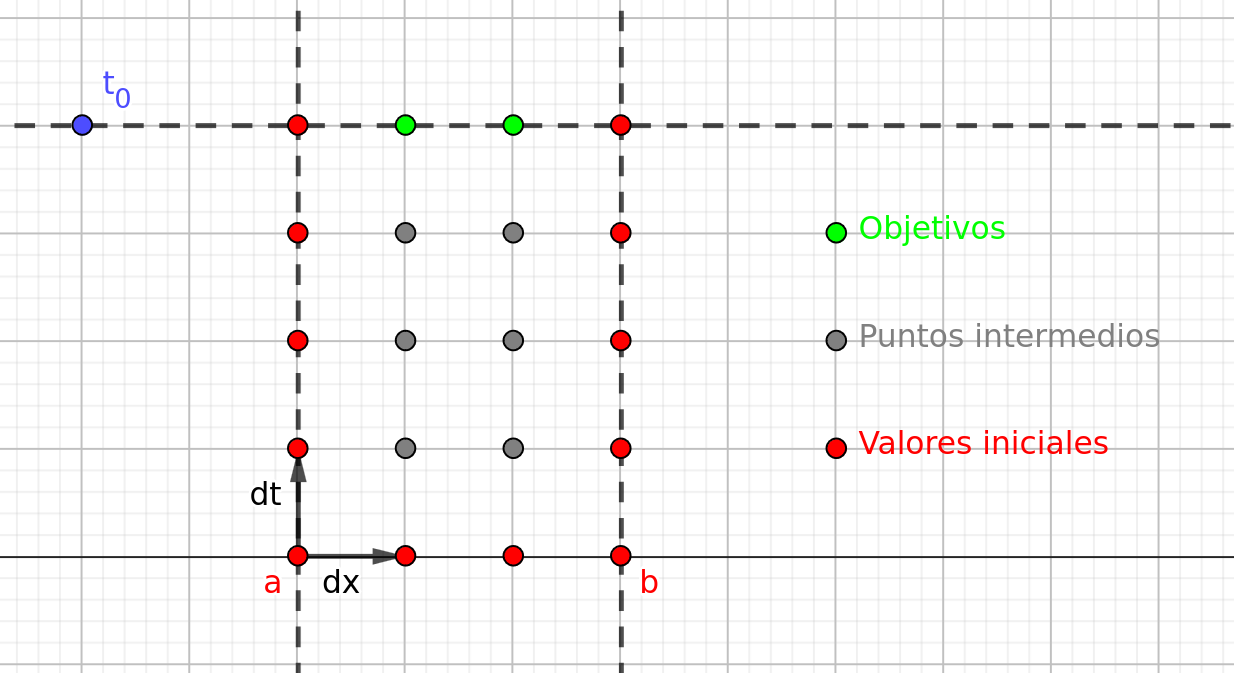
\includegraphics[scale=0.25]{./Imagenes/Bitmap/1dheatpoints.png}
	\caption{Representación en la malla del esquema \eqref{eq:1dheat_formula}}
	\label{fig:1d_grid}
\end{figure}

Antes de estudiar la convergencia de \eqref{eq:1dheat_formula}, presentamos el siguiente lema:

\begin{lema}\label{lema:1dheat}
	Suponiendo que $u$ tres veces diferenciable respecto de la variable $x$, si definimos el error de truncamiento como
	\begin{equation}
		\label{eq:lema1_eq1}
		\tau(x,t):= u^t(x,t)-u^{x\bar{x}}(x,t),
	\end{equation}
	se tiene que
	\begin{equation}
		\tau(x,t) \xrightarrow[\Delta x \rightarrow 0, \Delta t\rightarrow 0]{} 0.
	\end{equation}
	
\end{lema}

\begin{proof}
	Utilizando los lemas \ref{lema:error_prog} y \ref{lema:error_segunda}, se tiene que
	\begin{equation}
		\tau(x,t) := u^{t}(x,t) - u^{x\bar{x}}(x,t) = \frac{\partial^2u}{\partial x^2} - \frac{\partial u}{\partial t} + h^1(\Delta t) - h^2(\Delta x).
	\end{equation}
	Se sigue de \eqref{eq:1dheat} que
	\begin{equation}
		\tau(x,t) = h^1(\Delta t) - h^2(\Delta x),
	\end{equation}
	y como las funciones $h^1$ y $h^2$ tienden a 0 cuando $\Delta t$ y $\Delta x$ tienden a 0 respectivamente, es claro que $\tau(x,t)$ tiende a 0 cuando hacemos la malla más pequeña.
\end{proof}

\com{En el siguiente teorema me preguntas quién es $\tau_{i,j}$. En la sección \ref{sec:notacion} (que ahora he movido de sitio) explicito que significa $f_{i,j}$ para cualquier función $f$.}


\begin{teorema}
	Si $0<\lambda<\frac{1}{2}$, el método numérico \eqref{eq:1dheat_formula} es convergente\footnote{De hecho, el método converge si y solo si $0<\lambda<\frac{1}{2}$, pero no lo probaremos por que solo nos interesa cuándo converge}, o dicho de otra forma, si definimos el error de aproximación del método $\epsilon_{i,j}:=|u_{i,j}-U_{i,j}|$, $\sup_{i,j}\epsilon(i,j)\rightarrow0$ si $\Delta t, \Delta x \rightarrow 0$.
\end{teorema}

\begin{proof}
	Teniendo en cuenta el lema anterior, si ahora repetimos las cuentas que nos llevaron a \eqref{eq:1dheat_formula} pero para $u$ en lugar de para $U$, obtenemos la ecuación
	\begin{equation}
		u_{i,j+1} = (1-2\lambda)u_{i,j}+\lambda(u_{i-1,j}+u_{i+1,j})+\Delta t\tau_{i,j},
	\end{equation}
	por lo que
	\begin{gather}
		\epsilon_{i,j+1} = |u_{i,j+1}-U_{i,j+1}| = \\ |((1-2\lambda)u_{i,j}+\lambda(u_{i-1,j}+u_{i+1,j})+\Delta t\tau_{i,j}) \\
		 - ((1-2\lambda)U_{i,j}+\lambda(U_{i-1,j}+U_{i+1,j}))| = \\
		 |(1-2\lambda)(u_{i,j}-U_{i,j})+\lambda(u_{i+1,j}-U_{i+1,j}+u_{i-1,j}-U_{i-1,j}) + \Delta t\tau_{i,j}|.
	\end{gather}
	Utilizando la desigualdad triangular, obtenemos
	\begin{multline}
		\epsilon_{i,j+1} \leq (1-2\lambda)|u_{i,j}-U_{i,j}|+\lambda(|u_{i+1,j}-U_{i+1,j}|+|u_{i-1,j}-U_{i-1,j}|) + \Delta t|\tau_{i,j}| \\
		= (1-2\lambda)\epsilon_{i,j}+\lambda(\epsilon_{i+1,j}+\epsilon_{i-1,j}) + \Delta t|\tau_{i,j}|.
	\end{multline}
	Ahora, si definimos
	\begin{equation}
		E_j:=\sup_{i}|\epsilon_{i,j}|\hspace{30px}\tau:=\sup_{i,j}|\tau_{i,j}|
	\end{equation}
	tenemos que
	\begin{equation}
		E_{j+1}\leq E_j+\Delta t\tau,
	\end{equation}
	mediante una inducción trivial concluimos que
	\begin{equation}
		E_j \leq E_0 + j\Delta t\tau = E_0+t_j\tau = t_j\tau,\hspace{15px}\forall j\geq0
	\end{equation}
	donde $E_0$ es el supremo del error en $t=0$ (que es $0$ porque $U_{i,0} =f(x_i)= u_{i,0}$ por definición).
	
	Con esto hemnos acabado la demostración, pues está claro (por su definición) que $\tau$ tiende a 0 cuando $\Delta t, \Delta x$ tienden a 0, luego el error está acotado por algo que tiende a 0, lo que implica que tiende a 0.
\end{proof}

\section{Ecuación del calor en dos dimensiones}


En el caso bidimensional, la ecuación depende de un parámetro $\kappa\geq0$, \comp{La verdad es que no encontré un resultado que me asegurara que en dos dimensiones podía hacer ese cambio de variable así que seguí con él, no es porque prefiera mantenerlo} y tiene la siguiente forma
\begin{equation}
	\frac{\partial u}{\partial t}=\kappa\left(\frac{\partial^2u}{\partial x^2}+\frac{\partial^2u}{\partial y^2}\right)
\end{equation}
Al igual que en el caso lineal, pediremos unas condiciones de valor inicial y frontera para asegurar la existencia y unicidad de las soluciones, el problema concreto sería:
\begin{equation}\label{eq:2dheat}
	\begin{cases} 
			\frac{\partial u}{\partial t}(x,y,t) =\kappa\left(\frac{\partial^2u}{\partial x^2}(x,y,t)+\frac{\partial^2u}{\partial y^2}(x,y,t)\right), & a\leq x\leq b, \hspace{5px}, c \leq y \leq d, \hspace{5px} 0\leq t \leq T,\\
		u(x,y,0)=f(x,y), & a\leq x\leq b, \hspace{5px}, c \leq y \leq d, \\
		u(a,y,t)=\alpha(y,t), & c \leq y \leq d \hspace{5px}, 0<t,\\
		u(b,y,t)=\beta(y,t), & c \leq y \leq d \hspace{5px}, 0<t,\\
		u(x,c,t)=\gamma(x,t), & a < x < b \hspace{5px}, 0<t\leq T,\\
		u(x,d,t)=\delta(x,t), & c < y < d \hspace{5px}, 0<t\leq T.
	\end{cases}
\end{equation}

Dada la definición, queda claro que el dominio con el que trabajamos será el ortoedro $R:=\{(x,y,t) \hspace{5px} | \hspace{5px} a \leq x \leq b, \hspace{5px} c\leq y \leq d, \hspace{5px} 0\leq t \leq T\}$.

\subsection{Existencia y unicidad}
En \cite[pg. 66]{2deq} podemos encontrar el siguiente resultado que utilizaremos para demostrar la unicidad de la solución:

\com{En el libro que me recomendaste, el Weinberger, solo aparecía la demostración para una y tres dimensiones, por eso he tenido que hacer un poco este apaño. No obstante, si me pudieras decir algún lugar donde encontrar la demostración para dos dimensiones, estaría más que encantada de no complicarme la vida.}
\begin{teorema}
	Sea $D$ un dominio tridimensional limitado por una superficie cerrada $C$. Si existe, la solución del problema
	\[
	\begin{split}
		\frac{\partial u}{\partial t} - \kappa \left(\frac{\partial^2 u}{\partial x^2} + \frac{\partial^2 u}{\partial y^2} + \frac{\partial^2 u}{\partial z^2}\right) &= F(x,y,z,t) \hspace{15px} 	\text{en } D \\
		u(x,y,z,0) &= g(x,y,z) \hspace{15px} \text{en } D\\
		u(x,y,z,t) &= h(x,y,z,t) \hspace{15px} \text{sobre } C
	\end{split}
	\]
	es única.
\end{teorema}

\begin{teorema}[Existencia y unicidad]
	El problema \eqref{eq:2dheat} tiene solución y esta es única.
\end{teorema}
\begin{proof}
	La solución del problema puede calcularse mediante la técnica de separación de variables, puede encontrarse los cálculos concretos en \cite{2dheatexistence}. Solo nos queda pues demostrar la unicidad.
	
	El Teorema anterior nos garantiza la unicidad de la solución para la ecuación del calor no homogénea en tres dimensiones sobre un dominio cerrado, pero la ecuación del calor en dos dimensiones homogénea (osea, $F=0$), puede obtenerse como un caso particular de la de tres dimensiones, ajustando las funciones para que la temperatura no dependa del valor de $z$ (y por tanto obteniendo que $\frac{\partial^2u}{\partial z^2}=0$), lo que prueba la unicidad de la solución.
\end{proof}

\subsection{Aproximación de la solución}
\com{
El tema de los índices y del error igual que en la sección anterior.
}
Teniendo en cuenta la notación descrita en la Sección \ref{sec:notacion}, así como la definición \ref{def:malla3d}, vamos a aproximar la solución por la función $U$ en los puntos de la malla $M^3(a,b,c,d,0,T,n_x,n_y,n_t)$, que a partir de ahora denotaremos simplemente como $M$. Es sencillo ver que para el dominio de este problema concreto $(x_i,y_j,t_k)\in R \iff 0\leq i < n_x, \hspace{5px} 0\leq j < n_y, \hspace{5px} 0 \leq k < n_t$.

Vamos a hacer una aproximación completamente análoga a la aproximación de la versión lineal de esta ecuación. La función de aproximación $U$ tendrá que cumplir la versión discreta de la ecuación $\frac{\partial u}{\partial t}=\kappa(\frac{\partial^2u}{\partial x^2}+\frac{\partial^2u}{\partial y^2})$ sustituyendo con las diferencias finitas \eqref{eq:not_ford} y \eqref{eq:not_second}, lo que nos lleva a
\begin{multline}
	U^t(x,y,t)=\kappa\left(U^{x\bar{x}}(x,y,t)+U^{y\bar{y}}(x,y,t)\right) \Rightarrow 
	\frac{U(x,y,t+\Delta t)-U(x,y,t)}{\Delta t} = \\ \frac{\kappa}{\Delta x^2}[U(x+\Delta x,y,t) - 2U(x,y,t) + U(x-\Delta x,y,t)] + \\ \frac{\kappa}{\Delta y^2}[U(x,y+\Delta y,t) -2U(x,y,t) + U(x,y + \Delta y, t)].
\end{multline}

Sean ahora $i,j,k$ tales que $x=x_i$, $y=y_j$ y $t=t_k$, podemos volver a escribir la ecuación anterior como 
\begin{equation}
	\frac{U_{i,j,k+1}-U_{i,j,k}}{\Delta t} = \frac{\kappa}{\Delta x^2}\left[ U_{i+1,j,k} - 2U_{i,j,k} + U_{i-1,j,k} \right] + \frac{\kappa}{\Delta y^2}\left[ U_{i,j+1,k} - 2U_{i,j,k} + U_{i-1,j,k}\right],
\end{equation}
que, si definimos $\lambda_x:=\frac{\kappa\Delta t}{\Delta x^2}$ y $\lambda_y:= \frac{\kappa \Delta t}{\Delta x^2}$ y despejamos, nos lleva a la fórmula explícita
\begin{equation}\label{eq:2dheat_formula}
	U_{i,j,k+1} = \lambda_x(U_{i+1,j,k} + U_{i-1,j,k}) + \lambda_y( U_{i,j+1,k} + U_{i,j-1,k}) + \left(1 - 2\lambda_x -2\lambda_y \right)U_{i,j,k}.
\end{equation}

La fórmula \eqref{eq:2dheat_formula} nos permite calcular el valor de $U$ en un tiempo $t_k$ siempre que conozcamos el valor de la función en el tiempo $t_{k-1}$ en cualquier punto en el interior del rectángulo (en la frontera no es importante aproximar la función, ya que gracias a las condiciones de \eqref{eq:2dheat} sabemos su valor exacto).

Hagamos ahora las siguientes definiciones:
\begin{equation}
	\begin{cases}
		U_{i,j,0}:= f(a+i\Delta x,c+j\Delta y), & \forall (i,j) \in \{0,\dots,n_x-1\} \times \{0, \dots, n_y-1\}, \\
		U_{0,j,k}:=\alpha(c+j\Delta y,k\Delta t), & \forall (j,k) \in \{0,\dots, n_y-1\}\times \{1,\dots, n_t-1\}, \\
		U_{n_x-1,j,k}:= \beta(c+j\Delta y,k\Delta t), & \forall (j,k) \in \{0,\dots, n_y-1\}\times \{1,\dots, n_t-1\}, \\
		U_{i,0,k}:= \gamma(a+i\Delta x,k\Delta t), & \forall (i,k) \in \{1, \dots, n_x-2\} \times \{1, \dots, n_t-1\}, \\
		U_{i,n_y-1,k}:= \delta(a+i\Delta x,k\Delta t), & \forall (i,k) \in \{1, \dots, n_x-2\} \times \{1, \dots, n_t-1\}.
	\end{cases}
\end{equation}

Es fácil observar que utilizándolas como casos base para la fórmula \eqref{eq:2dheat_formula}, podemos calcular el valor de $U$ en todos los puntos de la malla. En general, supondremos que el objetivo es aproximar los valores de $u(x,y,T)$ en los puntos de la malla que proceden, osea calcular los valores $U_{i,j,n_t-1} \hspace{5px} \forall (i,j)\in\{1,\dots,n_x-2\} \times \{1,\dots, n_y-2\}$. Podemos observar una representación a pequeña escala de qué puntos tenemos y cuales necesitamos en la Figura \ref{fig:2dheatpoints}.

\begin{figure}
	\centering
	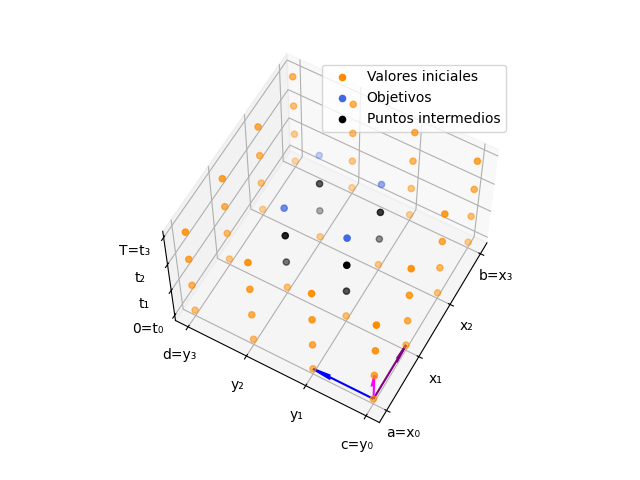
\includegraphics[scale=0.7]{./Imagenes/Bitmap/2dheatpoints.png}
	\caption{Representación en la malla del esquema \eqref{eq:2dheat_formula}, siendo los vectores azul, rosa y morado los valores $\Delta y$, $\Delta t$ y $\Delta x$ respectivamente. \comp{Estoy de acuerdo en que no es muy clara la imagen, pero genuninamente no sé como hacerla más clara. ¿Algún consejo al respecto?}}
	\label{fig:2dheatpoints}
\end{figure}

Antes de estudiar la convergencia del esquema, necesitamos extrapolar el resultado obtenido en el Lema \ref{lema:1dheat} a la ecuación sobre el plano.

\begin{lema}
		Suponiendo que $u$ es tres veces diferenciable en las variables $x$ e $y$, si definimos el error de truncamiento como:
	\begin{equation}
		\label{eq:lema2_eq1}
		\tau(x,y,t) := u^t(x,y,t)-\kappa \left(u^{x\bar{x}}(x,y,t) + u^{y\bar{y}}(x,y,t)\right),
	\end{equation}
	se tiene que
	\begin{equation}
		\tau_(x,y,t) \xrightarrow[\Delta x \rightarrow 0, \Delta y\rightarrow 0 \Delta t\rightarrow 0]{} 0.
	\end{equation}
\end{lema}

\begin{proof}
	Aplicando los lemas \ref{lema:error_prog} y \ref{lema:error_segunda}, podemos ver que
	\begin{multline}
		\tau(x,y,t) := u^t(x,y,t)-\kappa \left(u^{x\bar{x}}(x,y,t) + u^{y\bar{y}}(x,y,t)\right) = \\
		-\frac{\partial u}{\partial t} + \kappa\left( \frac{\partial^2u}{\partial x^2} + \frac{\partial^2u}{\partial y^2}\right) + h^1(\Delta t) - \kappa(h^2(\Delta x) + h^3(\Delta y)  = \\ h^1(\Delta t) - \kappa(h^2(\Delta x) + h^3(\Delta y)).	
	\end{multline}
	Es inmediato ver que $\tau(x,y,t)$ tiende a 0 cuando hacemos la malla más fina, dado que las funciones $h^i$ tienden a 0 también tienden a 0 cuando hacemos la malla más fina.
\end{proof}

\begin{teorema}
	Si $0<\lambda_x + \lambda_y<\frac{1}{2}$, el método numérico \eqref{eq:2dheat_formula} es convergente, o dicho de otra forma, si definimos el error de aproximación del método $\epsilon_{i,j,k}.=|u_{i,j,k}-U_{i,j,k}|$, $sup_{i,j,k}\epsilon_{i,j,k}\rightarrow 0$ si $\Delta t,\Delta x,\Delta y \rightarrow 0$.
\end{teorema}
\begin{proof}
	Teniendo en cuenta el lema anterior, si ahora repetimos las cuentas que nos llevaron a \eqref{eq:2dheat_formula} pero para $u$ en lugar de para $U$, obtenemos la ecuación
	\begin{equation}
		u_{i,j,k+1} = (1-2\lambda_x -2\lambda_y) u_{i,j,k}+ \lambda_x(u_{i-1,j,k}+u_{i+1,j,k}) + \lambda_y(u_{i,j-1,k} +u_{i,j+1,k}) +\Delta t\tau_{i,j,k},
	\end{equation}
	por lo que
	\begin{gather}
		\epsilon_{i,j,k+1} = |u_{i,j+1}-U_{i,j+1}| = \\ |\left[(1-2\lambda_x-2\lambda_y)u_{i,j,k}+\lambda_x(u_{i-1,j,k}+u_{i+1,j,k})+ \lambda_y(u_{i,j-1,k} +u_{i,j+1,k}) + \Delta t\tau_{i,j,k}\right] \\ 
		- \left[(1-2\lambda_x-2\lambda_y) U_{i,j,k}+\lambda_x(U_{i-1,j,k}+U_{i+1,j,k}) + \lambda_y(U_{i,j-1,k} +U_{i,j+1,k})\right]| = \\
		|(1-2\lambda_x -2\lambda_y)(u_{i,j,k}-U_{i,j,k}) +\lambda_x(u_{i+1,j,k}-U_{i+1,j,k}+u_{i-1,j,k}-U_{i-1,j,k}) + \\ 
		\lambda_y(u_{i,j+1,k}-U_{i,j+1,k}+u_{i,j-1,k}-U_{i,j-1,k})
		\Delta t\tau_{i,j,k}|.
	\end{gather}
	Utilizando la desigualdad triangular, obtenemos
	\begin{multline}
		\epsilon_{i,j,k+1} \leq (1-2\lambda_x-2\lambda_y)|u_{i,j,k}-U_{i,j,k}|+\lambda_x(|u_{i+1,j,k}-U_{i+1,j,k}|+|u_{i-1,j,k}-U_{i-1,j,k}|) + \\ \lambda_y(|u_{i,j+1,k}-U_{i,j+1,k}|+|u_{i,j-1,k}-U_{i,j-1,k}|) + \Delta t|\tau_{i,j,k}| \\
		= (1-2\lambda_x-2\lambda_y)\epsilon_{i,j,k}+\lambda_x(\epsilon_{i+1,j,k}+\epsilon_{i-1,j,k}) +\lambda_y(\epsilon_{i,j+1,k}+\epsilon_{i,j-1,k}) + \Delta t|\tau_{i,j,k}|.
	\end{multline}
	Ahora, si definimos
	\begin{equation}
		E_k:=\sup_{i,j}|\epsilon_{i,j,k}|\hspace{30px}\tau:=\sup_{i,j}|\tau_{i,j,k}|
	\end{equation}
	tenemos que
	\begin{equation}
		E_{k+1}\leq E_k+\Delta t\tau,
	\end{equation}
	mediante una inducción trivial concluimos que
	\begin{equation}
		E_k \leq E_0 + k\Delta t\tau = E_0+t_k\tau = t_k\tau,\hspace{15px}\forall k\geq0
	\end{equation}
	donde $E_0$ es el supremo del error en $t=0$ (que es $0$ porque $U_{i,j,0} =f(x_i,y_j)= u_{i,j,0}$ por definición).
	
	Con esto hemos acabado la demostración, pues está claro (por su definición) que $\tau$ tiende a 0 cuando $\Delta t, \Delta x, \Delta y$ tienden a 0, luego el error está acotado por algo que tiende a 0, lo que implica que tiende a 0.
\end{proof}